%%\documentclass[a4paper,12pt,oneside]{llncs}
\documentclass[12pt,letterpaper]{article}
\usepackage[right=2cm,left=3cm,top=2cm,bottom=2cm,headsep=0cm]{geometry}

%%%%%%%%%%%%%%%%%%%%%%%%%%%%%%%%%%%%%%%%%%%%%%%%%%%%%%%%%%%
%% Juego de caracteres usado en el archivo fuente: UTF-8
\usepackage{ucs}
\usepackage[utf8x]{inputenc}

%%%%%%%%%%%%%%%%%%%%%%%%%%%%%%%%%%%%%%%%%%%%%%%%%%%%%%%%%%%
%% Juego de caracteres usado en la salida dvi
%% Otra posibilidad: \usepackage{t1enc}
\usepackage[T1]{fontenc}

%%%%%%%%%%%%%%%%%%%%%%%%%%%%%%%%%%%%%%%%%%%%%%%%%%%%%%%%%%%
%% Ajusta maergenes para a4
%\usepackage{a4wide}

%%%%%%%%%%%%%%%%%%%%%%%%%%%%%%%%%%%%%%%%%%%%%%%%%%%%%%%%%%%
%% Uso fuente postscript times, para que los ps y pdf queden y pequeños...
\usepackage{times}

%%%%%%%%%%%%%%%%%%%%%%%%%%%%%%%%%%%%%%%%%%%%%%%%%%%%%%%%%%%
%% Posibilidad de hipertexto (especialmente en pdf)
%\usepackage{hyperref}
\usepackage[bookmarks = true, colorlinks=true, linkcolor = black, citecolor = black, menucolor = black, urlcolor = black]{hyperref}

%%%%%%%%%%%%%%%%%%%%%%%%%%%%%%%%%%%%%%%%%%%%%%%%%%%%%%%%%%%
%% Graficos 
\usepackage{graphics,graphicx}

%%%%%%%%%%%%%%%%%%%%%%%%%%%%%%%%%%%%%%%%%%%%%%%%%%%%%%%%%%%
%% Ciertos caracteres "raros"...
\usepackage{latexsym}

%%%%%%%%%%%%%%%%%%%%%%%%%%%%%%%%%%%%%%%%%%%%%%%%%%%%%%%%%%%
%% Matematicas aun más fuertes (american math dociety)
\usepackage{amsmath}

%%%%%%%%%%%%%%%%%%%%%%%%%%%%%%%%%%%%%%%%%%%%%%%%%%%%%%%%%%%
\usepackage{multirow} % para las tablas
\usepackage[spanish,es-tabla]{babel}

%%%%%%%%%%%%%%%%%%%%%%%%%%%%%%%%%%%%%%%%%%%%%%%%%%%%%%%%%%%
%% Fuentes matematicas lo mas compatibles posibles con postscript (times)
%% (Esto no funciona para todos los simbolos pero reduce mucho el tamaño del
%% pdf si hay muchas matamaticas....
\usepackage{mathptm}

%%% VARIOS:
%\usepackage{slashbox}
\usepackage{verbatim}
\usepackage{array}
\usepackage{listings}
\usepackage{multirow}

%% MARCA DE AGUA
%% Este package de "draft copy" NO funciona con pdflatex
%%\usepackage{draftcopy}
%% Este package de "draft copy" SI funciona con pdflatex
%%%\usepackage{pdfdraftcopy}
%%%%%%%%%%%%%%%%%%%%%%%%%%%%%%%%%%%%%%%%%%%%%%%%%%%%%%%%%%%
%% Indenteacion en español...
\usepackage[spanish]{babel}

\usepackage{listingsutf8}
% Para escribir código en C
% \begin{lstlisting}[language=C]
% #include <stdio.h>
% int main(int argc, char* argv[]) {
% puts("Hola mundo!");
% }
% \end{lstlisting}


\title{Práctica 4}
\author{Jesús Rodríguez Heras\\
	Arantzazu Otal Alberro\\
Roberto Muras González}

\begin{document}
	
	\maketitle
%	\begin{abstract} %Poner esto en todas las prácticas de PCTR
%%		\begin{center}
%%			\noindent
%			
%%		\end{center}
%	\end{abstract}
	\thispagestyle{empty}
	\newpage
	
%	\tableofcontents
%	\newpage
	
	%%\listoftables
	%%\newpage
	
	%%\listoffigures
	%%\newpage
	
	%%%% REAL WORK BEGINS HERE:
	
	%%Configuracion del paquete listings
	\lstset{language=bash, numbers=left, numberstyle=\tiny, numbersep=10pt, firstnumber=1, stepnumber=1, basicstyle=\small\ttfamily, tabsize=1, extendedchars=true, inputencoding=utf8/latin1, breaklines=true,literate=%
		{á}{{\'a}}1 %Esto es para que me pille la tilde de página en el ejemplo de index.html
	}
	
\section{Instalación de la máquina}
En esta primera parte vamos a crear el entorno de trabajo que utilizaremos durante la práctica. Para ello vamos a:
\begin{itemize}
	\item Iniciar una máquina Vagrant con una IP privada.
	\item Instalar apache.
	\item Instalar y configurar Webmin.
	\item Instalar php.
\end{itemize}

Para facilitar los ejercicios, se aconseja modificar el archivo host de la máquina anfitriona (portatil) para que pueda acceder al servidor mediante un nombre de dominio.

Instalación de apache:
\begin{center}
	\texttt{sudo apt-get install apache2}
\end{center}

Para instalar y configurar Webmin nos dirigimos a la página de descargas de Webmin para sistemas debian: \url{http://www.webmin.com/deb.html}

Nos dirigimos al apartado \textit{Using the webmin APT repository}. En el archivo \texttt{/etc/apt/sources.list} de la máquina virtual, pegamos lo siguiente:
\begin{center}
	\texttt{deb https://download.webmin.com/download/repository sarge contrib}
\end{center}

A continuación, actualizamos los paquetes e instalamos Webmin\footnote{Si nos da un fallo al hacer \texttt{sudo apt-get update} que nos dice que nos falta \texttt{apt-transport-https}, hacemos \texttt{sudo apt-get install apt-transport-https}.}.
\begin{center}
	\texttt{sudo apt-get update \&\& sudo apt-get install webmin}
\end{center}

Para instalar php, usamos el siguiente comando:
\begin{center}
	\texttt{sudo apt-get install php5-common}
	\texttt{sudo apt-get install libapache2-mod-php5}
\end{center}

A la hora de modificar el fichero \texttt{/etc/hosts} de la máquina anfitriona, lo abrimos con:
\begin{center}
	\texttt{sudo nano /etc/hosts}
\end{center}

Y añadimos la IP de la máquina virtual al final del archivo:
\begin{center}
	\texttt{192.168.1.100 manolorg.uca.es}
\end{center}

Siendo:
\begin{itemize}
	\item \texttt{192.168.1.100} la IP de la máquina virtual.
	\item \texttt{manolorg.uca.es} el dominio con el que vamos a trabajar.
\end{itemize}

Para comprobar que funciona, escribimos lo siguiente en el navegador de nuestro portátil:
\begin{center}
	\texttt{manolorg.uca.es}
\end{center}
\newpage
Y nos debe aparecer la página por defecto de apache.
\begin{figure}[h]
	\centering
	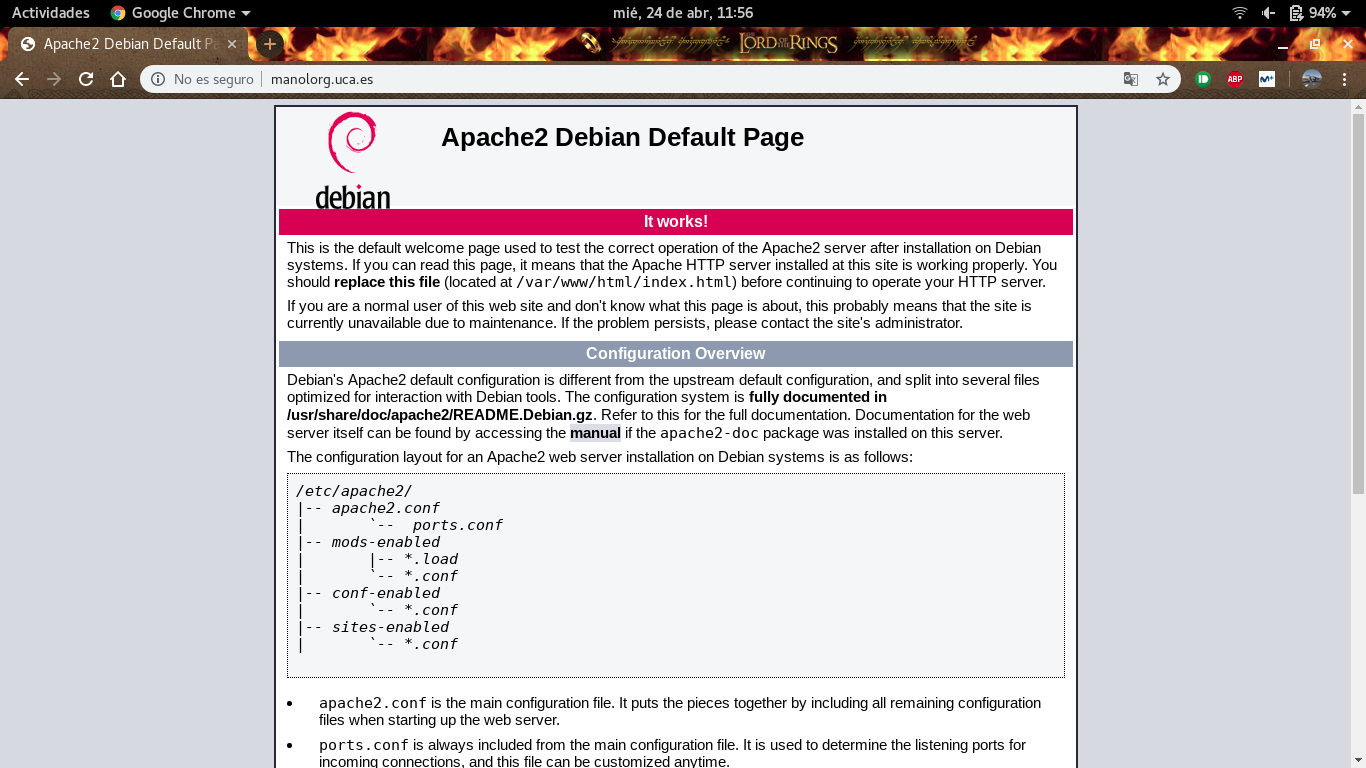
\includegraphics[scale=0.34]{Apache.png}
	\caption{Página inicial de Apache}
	\label{Página inicial de Apache}
\end{figure}

Para comprobar que Webmin está bien instalado, entramos en la siguiente dirección: 
\begin{center}
	\texttt{https://manolorg.uca.es:10000}
\end{center}
\begin{figure}[h]
	\centering
	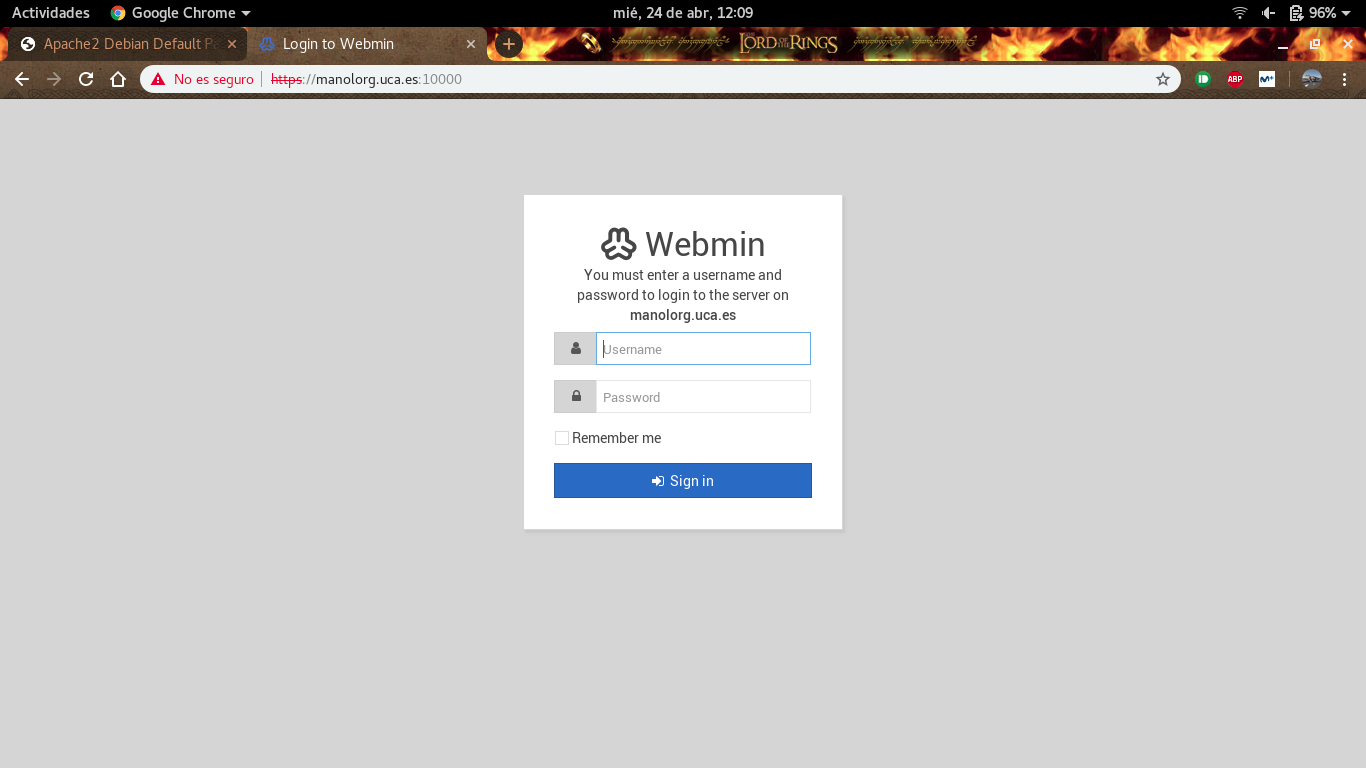
\includegraphics[scale=0.34]{Webmin.png}
	\caption{Página principal de Webmin}
	\label{Página principal de Webmin}
\end{figure}

\newpage
Para comprobar que php funciona bien cambiamos el archivo \texttt{/var/www/html/index.html} por \texttt{/var/www/html/index.php} y copiar el siguiente código en su interior:
\begin{lstlisting}[language=PHP]
<html>
  <head>
    <title>Prueba de PHP</title>
  </head>
  <body>
    <?php echo '<p>Hola Mundo</p>'; ?>
  </body>
</html>
\end{lstlisting}

Para ver si funciona, entramos en \texttt{manolorg.uca.es}.
\begin{figure}[h]
	\centering
	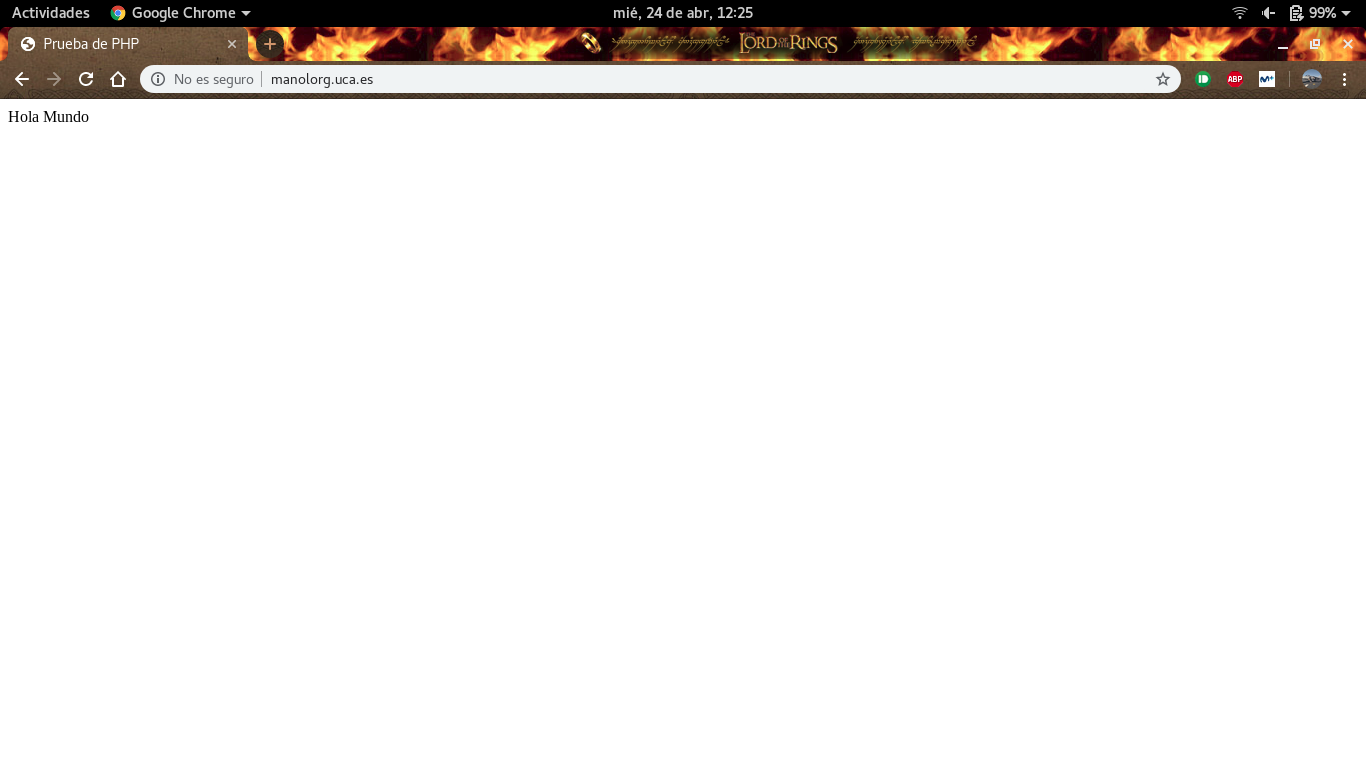
\includegraphics[scale=0.34]{PHP.png}
	\caption{Prueba PHP}
	\label{Prueba PHP}
\end{figure}

\newpage
\section{Configuración básica de apache}
Como ejemplo, vamos a modelar y configurar el entorno web del grupo de investigación Manolo Research Group.
\begin{itemize}
	\item La página principal del grupo está bajo el dominio \texttt{manolorg.uca.es}. El contenido se almacenará en \texttt{/var/www/manolorg}.
	
	Para ello accedemos a webmin y creamos un nuevo host virtual y, en document root ponemos \texttt{/var/www/manolorg}.
	
	\item Se desea que solo se acceda a la dirección \texttt{/docs} solo pueda acceder el usuario \texttt{admin} y el usuario \texttt{manolo}.
	
	Para ello creamos el directorio \texttt{/docs} y lo añadimos como ``directory'' en webmin. Luego, vamos a ``Access control'' y añadimos lo siguiente:
	\begin{itemize}
		\item En authentication realm name hay que poner algo (lo que sea).
		\item En restrict users by login poner ``All valid users''.
		\item En Authentication tipe, lo ponemos en basic.
		\item En clients must satisfy, ponemos ``All access control''.
		\item En User text file, ponemos el directorio del archivo txt (acceso.txt) con las contraseñas de los usuarios.
		\item En Basic login, en text file.	
		\item Guardamos y volvemos a entrar y podremos ver edit users. Y podremos crear el usuario que queramos.
	\end{itemize}
	
	\newpage
	Debería quedar como en la siguiente imagen\footnote{Solo deberíamos tener un fichero de constraseñas, que debería estar en el document root de \texttt{manolorg.uca.es}.}:
	\begin{figure}[h]
		\centering
		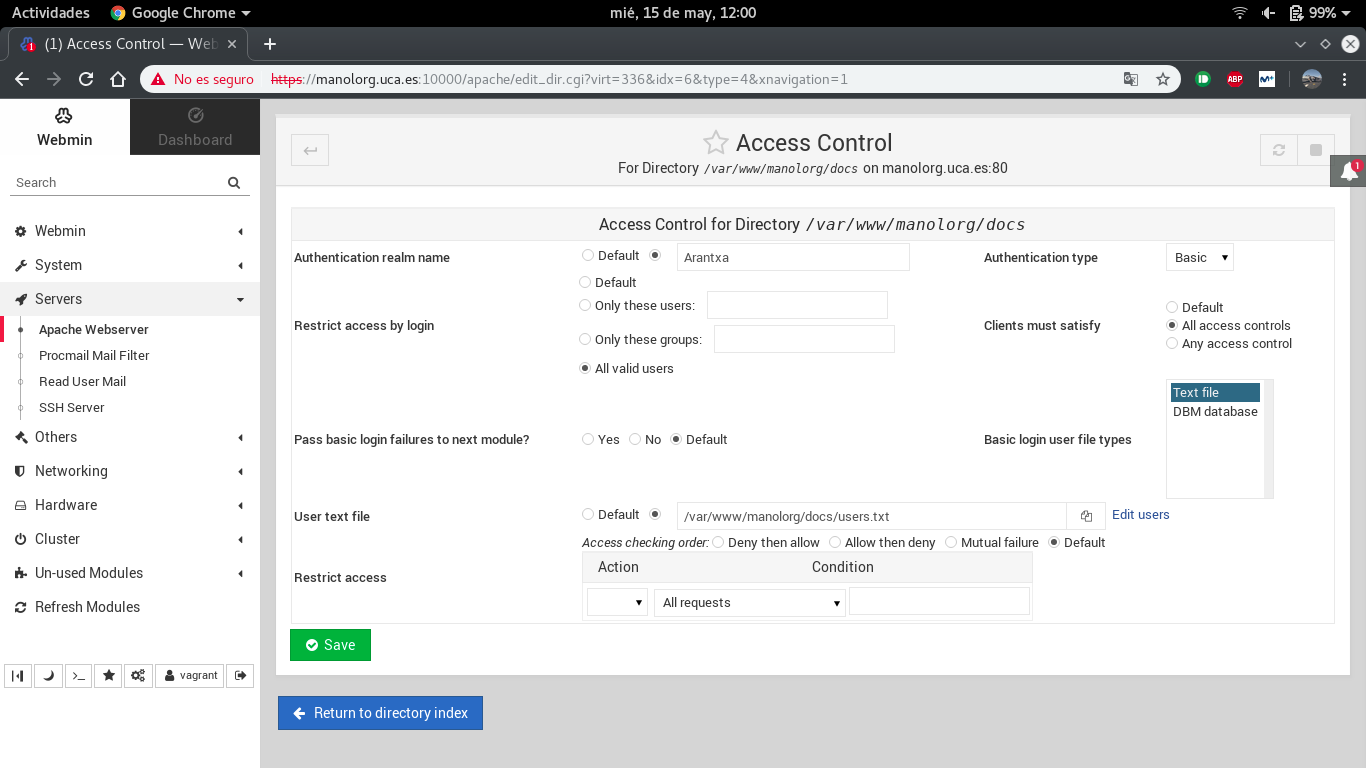
\includegraphics[scale=0.34]{ControlAcceso.png}
		\caption{Configuración de control de acceso.}
		\label{Configuración de control de acceso}
	\end{figure}

	Para crear el usuario con su contraseña, le damos al botón ``Edit Users'' que hay en ``Access Control'' y lo ponemos tal como vemos en la siguiente imagen:
	\newpage
	\begin{figure}[h]
		\centering
		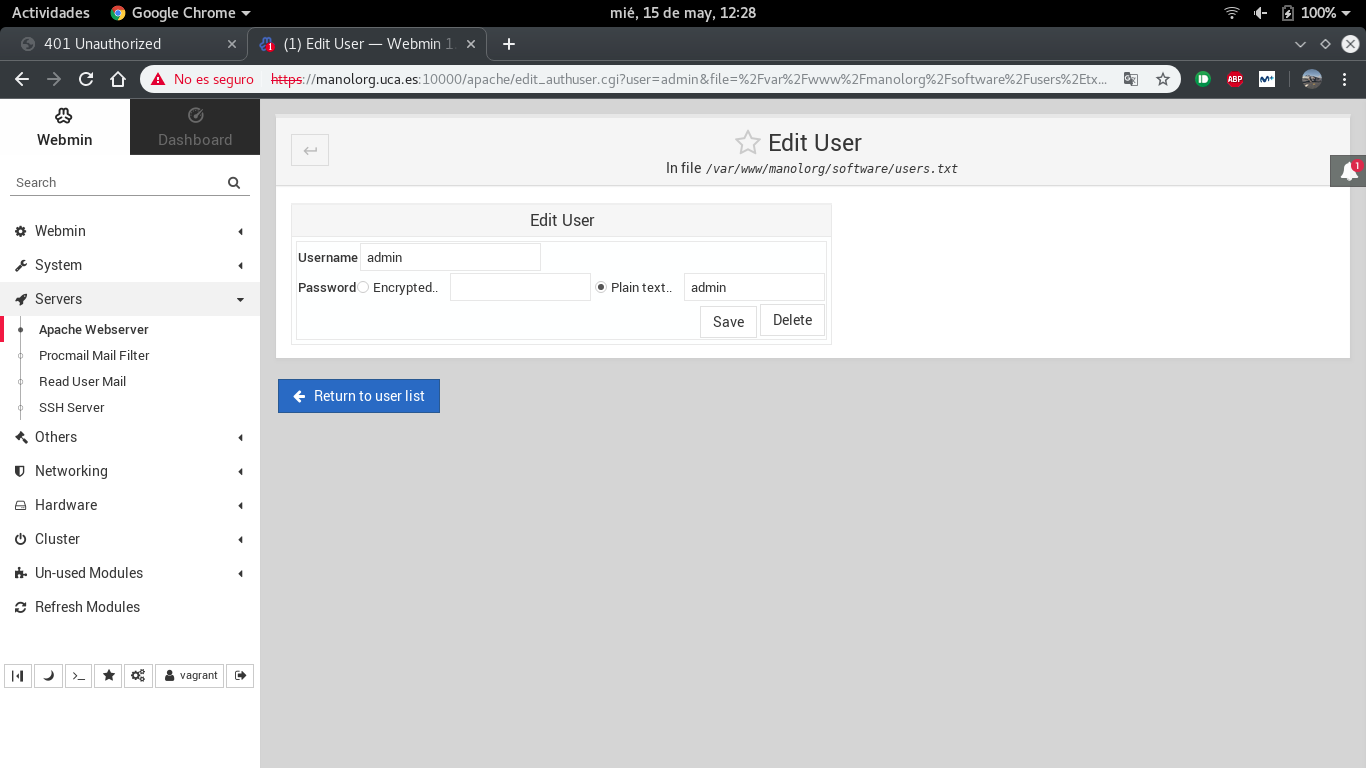
\includegraphics[scale=0.34]{Usuarios.png}
		\caption{Creación de usuarios.}
		\label{Creación de usuarios}
	\end{figure}

	Para comprobar si funciona entramos a la dirección \texttt{manolorg.uca.es/docs} y veremos que nos pide el control de acceso como en la siguiente imagen:
	\newpage
	\begin{figure}[h]
		\centering
		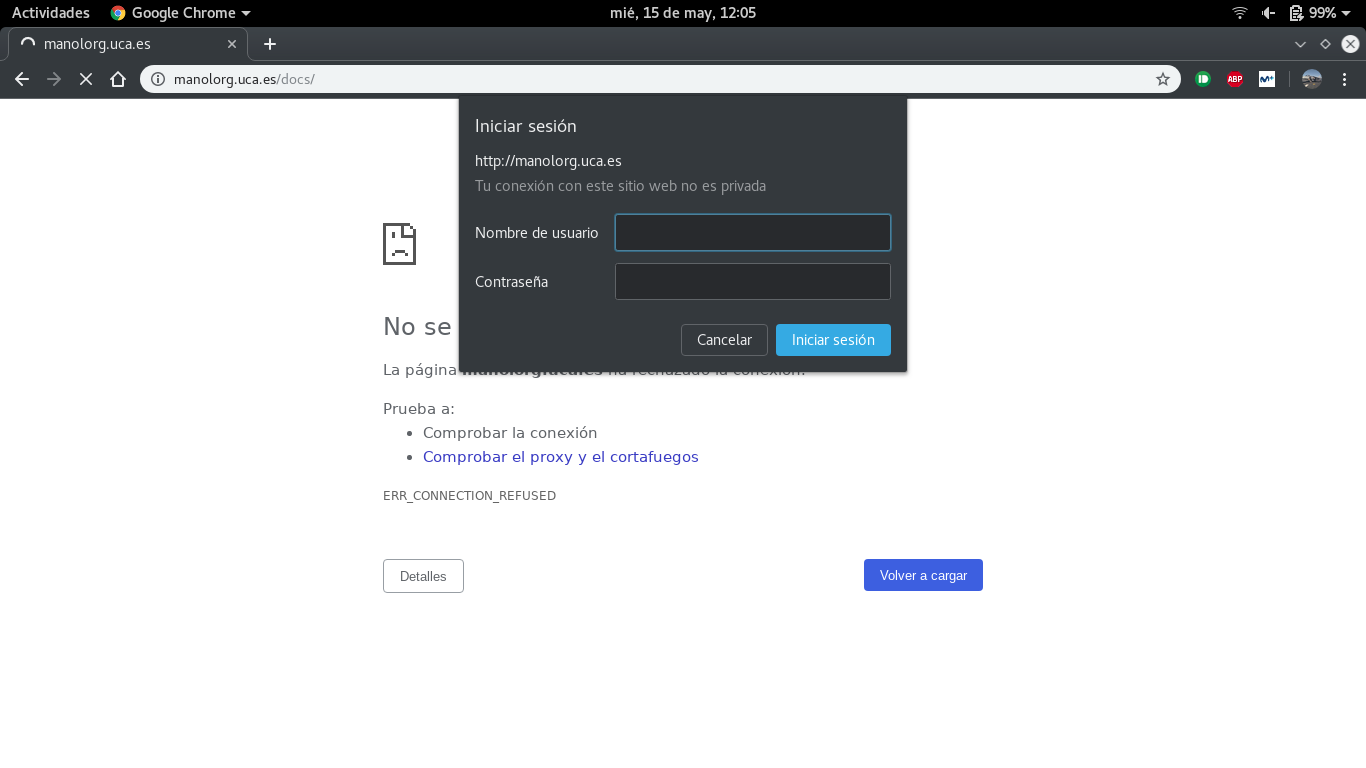
\includegraphics[scale=0.34]{Login.png}
		\caption{Configuración de control de acceso en \texttt{manolorg.uca.es/docs}.}
		\label{Configuración de control de acceso en manolorg.uca.es/docs}
	\end{figure}

	Si ponemos las credenciales creadas anteriormente, nos permitirá el acceso.
	
	\item No se mostrarán los directorios, excepto la carpeta \texttt{/software} que será solo accesible para el usuario \texttt{admin}.
	
	Para que el directorio \texttt{software} nos muestre el índice de archivos, tendremos que crear un nuevo ``directory'' llamado software, luego nos iremos al \texttt{Document Options} del nuevo directorio. Una vez ahí, tendremos que marcar la opción de ``Selected below'' y la opción ``Generate directory indexes'' como ``yes''. Quedaría como en la siguiente imagen:
	\newpage
	\begin{figure}[h]
		\centering
		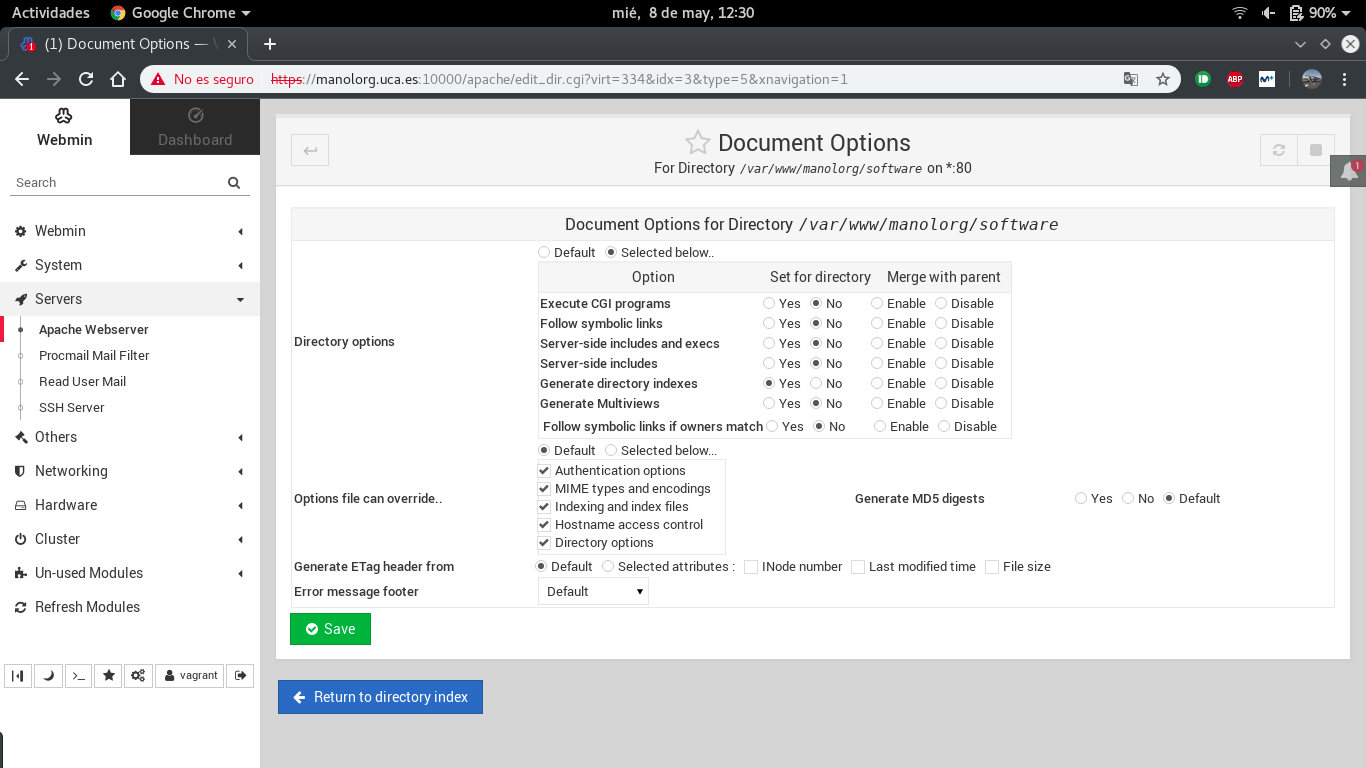
\includegraphics[scale=0.34]{Indexing.png}
		\caption{Document Options para software}
		\label{Document Options para software}
	\end{figure}

	También debemos configurar que solo tenga acceso el usuario admin en el ``Access Control''. Para ello, marcamos la opción ``Only these users'' como se ve en la siguiente imagen:
	\newpage
	\begin{figure}[h]
		\centering
		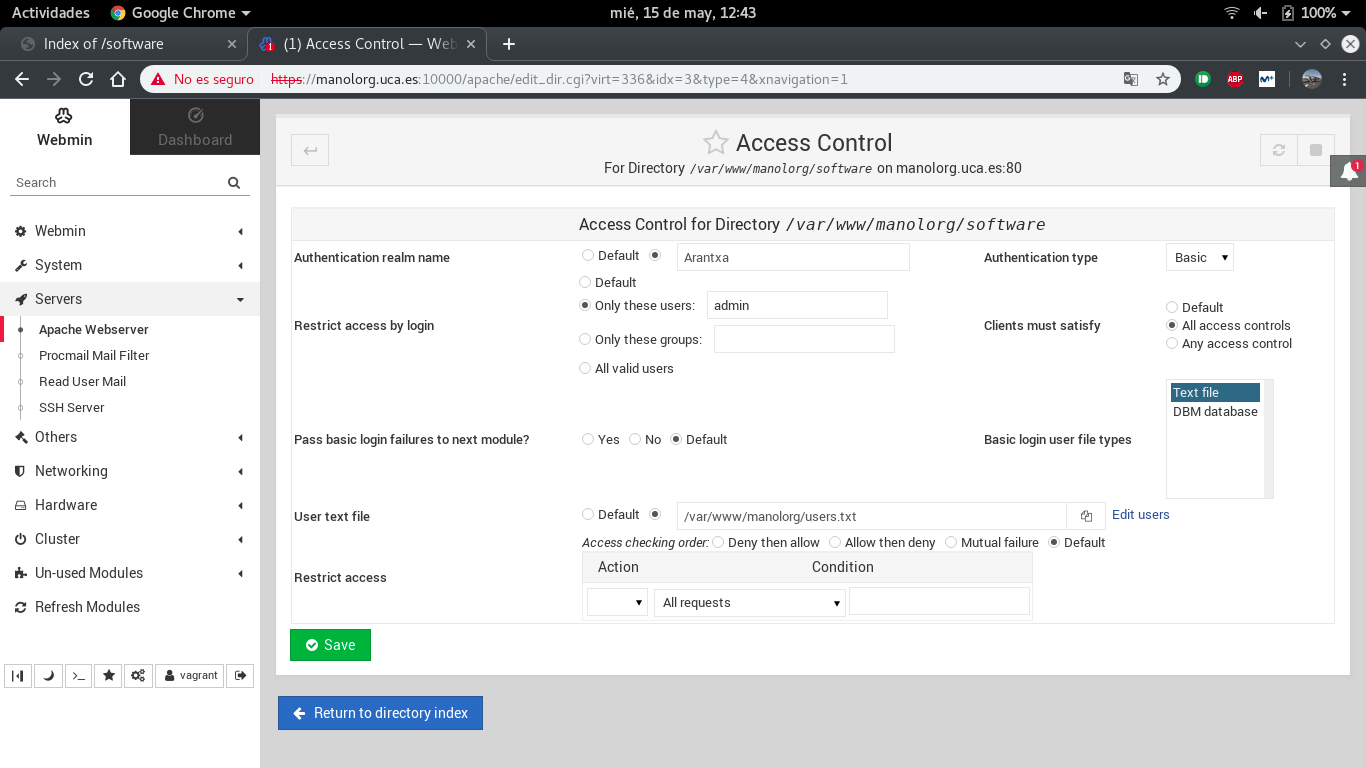
\includegraphics[scale=0.34]{Admin.png}
		\caption{Control de acceso para admin en \texttt{/software}.}
		\label{Control de acceso para admin en /software}
	\end{figure}
	
	\item La dirección \texttt{/sci2s} apuntará a la web \texttt{sci2s.ugr.es}.
	
	Para ello creamos el directory de \texttt{sci2s}, entramos dentro y le damos a ``Aliases and Redirects'' y ponemos la dirección deseada como en la siguiente imagen:
	\newpage
	\begin{figure}[h]
		\centering
		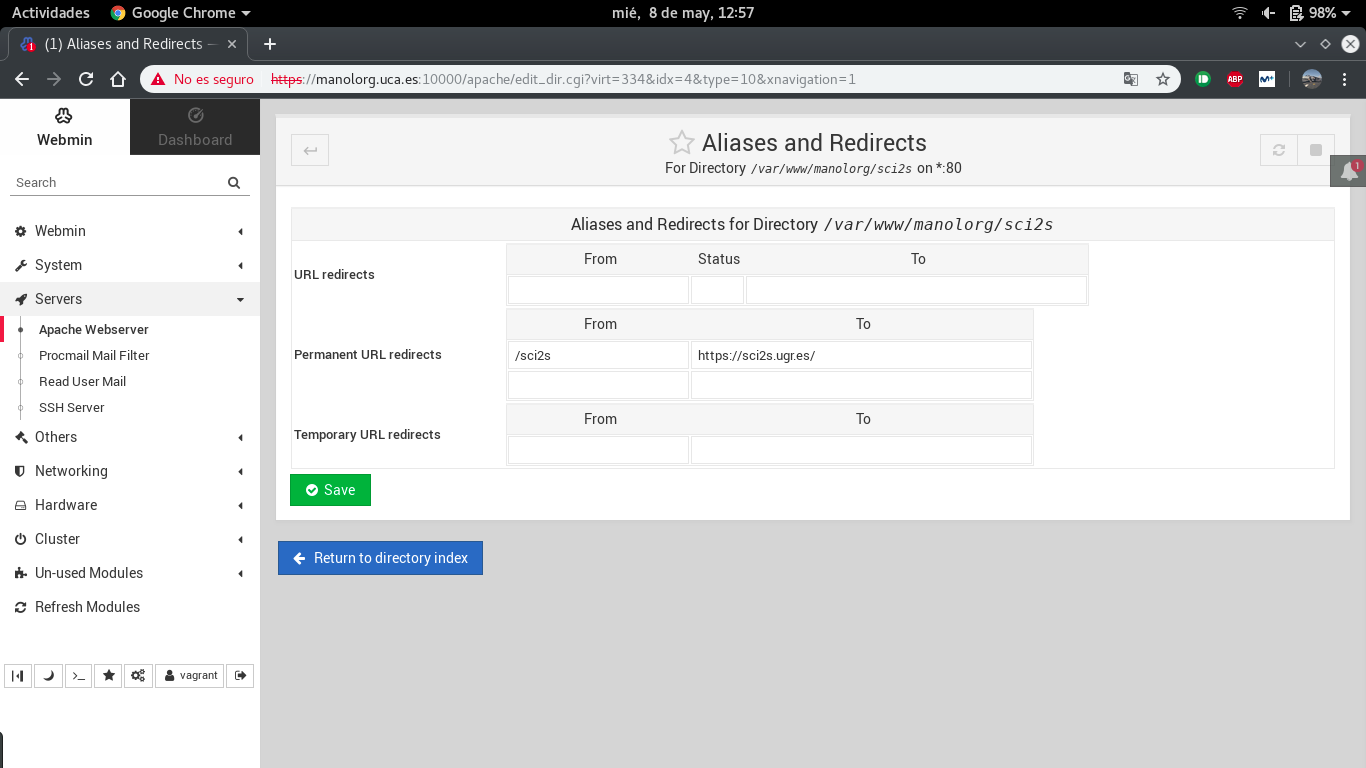
\includegraphics[scale=0.34]{ugr.png}
		\caption{Redirección a sci2s.ugr.es}
		\label{Redirección a sci2s.ugr.es}
	\end{figure}
	
	\item El grupo estará creado por diferentes laboratorios, crear un subdominio para el lab1 y el lab2. El contenido se almacenará en \texttt{/var/www/lab*}.
	
	Para ello, creamos dos carpetas nuevas desde la consola de la máquina virtual en \texttt{/var/www}, llamadas \texttt{lab1} y \texttt{lab2}.
	
	Para cada uno de los laboratorios, crearemos un virtual host distinto, y, en las opciones de creación, pondremos el document root en ``/var/www/labX'' (siendo X el número del laboratorio), pondremos el puerto 80, como \texttt{server name} pondremos ``labX.manolorg.uca.es'' (siendo X el número del laboratorio).
	
	\newpage
	\begin{figure}[h]
		\centering
		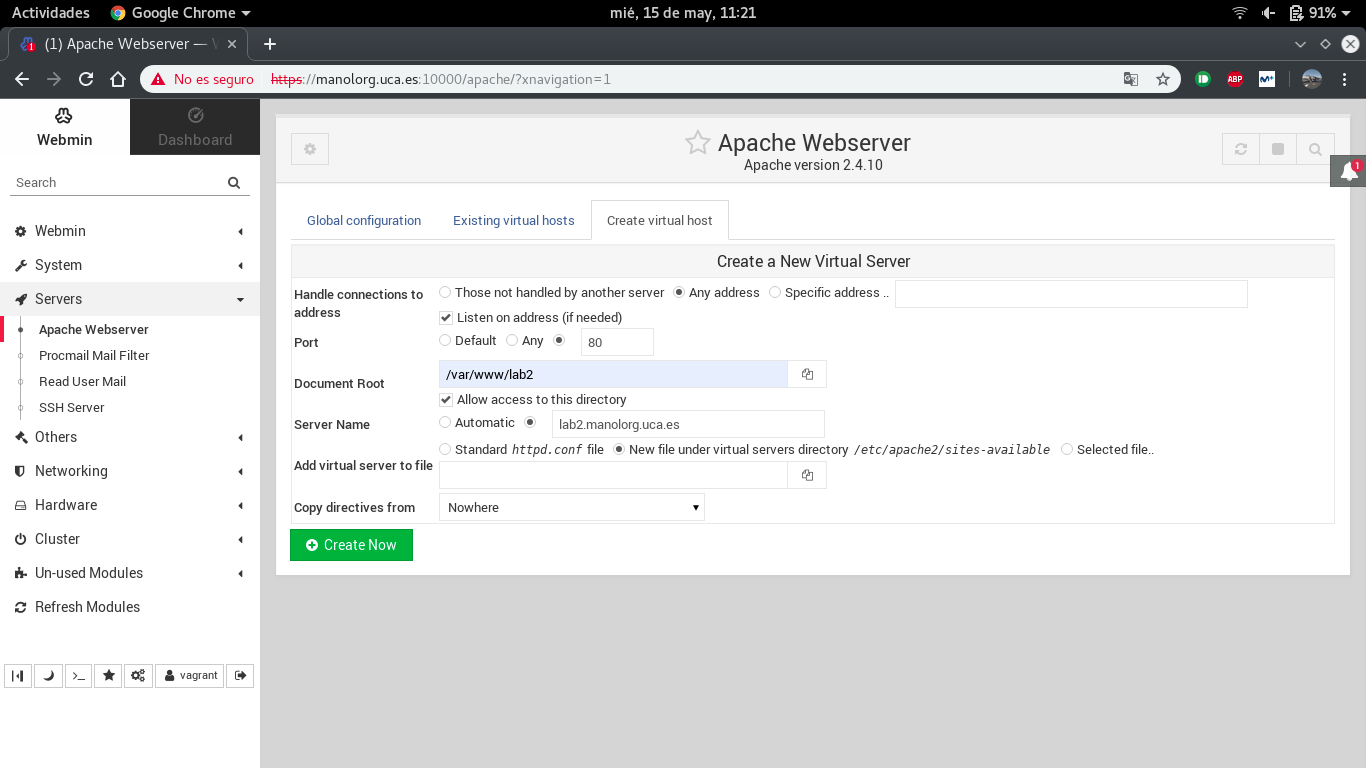
\includegraphics[scale=0.34]{CrearLab.png}
		\caption{Ejemplo de creación de \texttt{lab2.manolorg.uca.es}.}
		\label{Ejemplo de creación de lab2.manolorg.uca.es}
	\end{figure}
	
	Una vez hecho lo mismo con ambos laboratorios, entramos en \texttt{lab1.manolorg.uca.es} y \texttt{lab2.manolorg.uca.es} para ver si funcionan ambos sitios, tal como se muestra en la siguiente imagen:
	\begin{figure}[h]
		\centering
		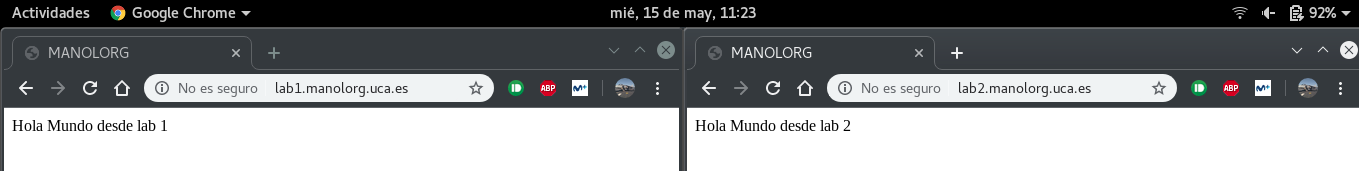
\includegraphics[scale=0.34]{FuncionanLabs.png}
		\caption{Muestra del funcionamiento de los laboratorios.}
		\label{Muestra del funcionamiento de los laboratorios}
	\end{figure}
\end{itemize}

Se deberá crear una web sencilla (Hola mundo) en cada uno de los dominios y carpetas. Las páginas deben tener caracteres con tildes, por lo que debemos configurar Apache para que trabaje con UTF8.

Para ello, usaremos el siguiente código en el fichero \texttt{/var/www/manolorg}:
\begin{lstlisting}[language=html]
<html>
	<head>
		<title>MANOLORG</title>
	</head>
	<body>
		<p>Página de inicio de manolorg.</p>
	</body>
</html>
\end{lstlisting}

\newpage
Por defecto, no funciona la codificación UTF8, como podemos ver en la siguiente imagen:
\begin{figure}[h]
	\centering
	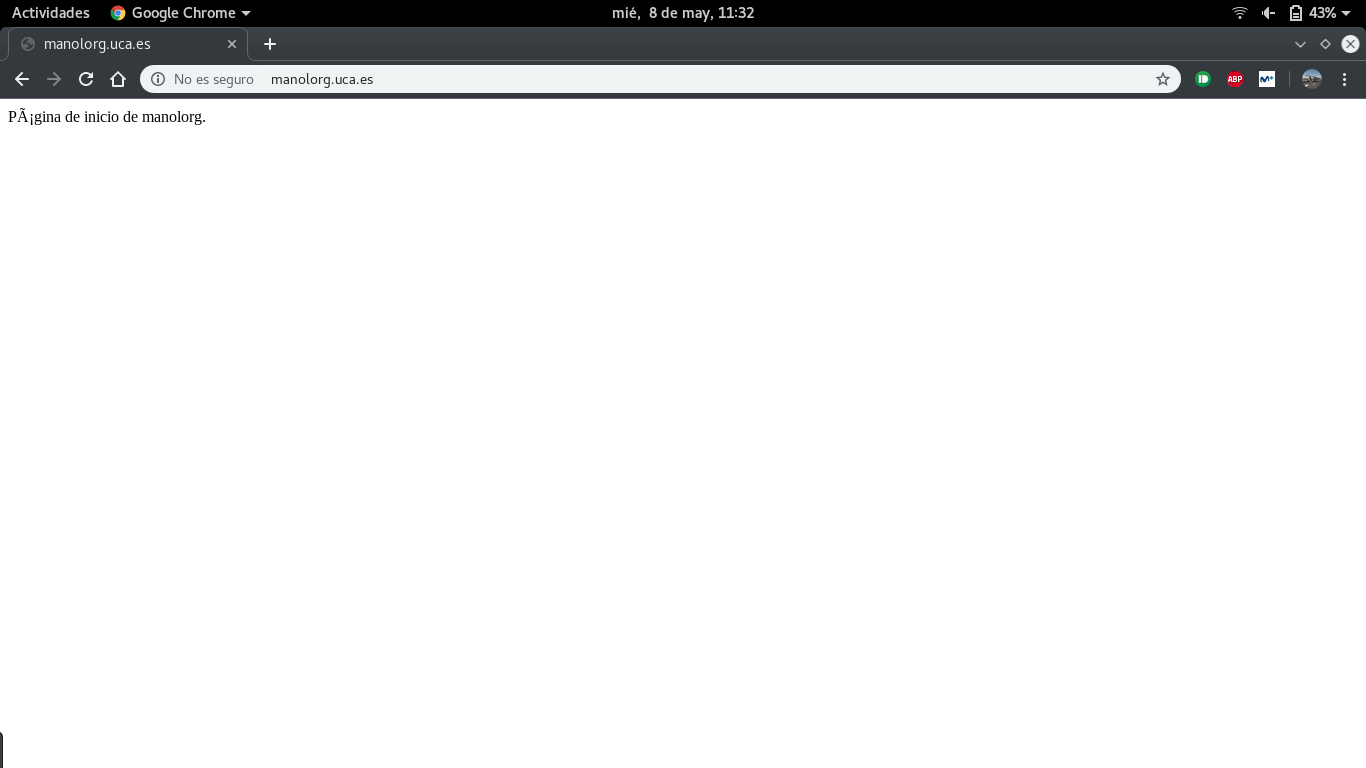
\includegraphics[scale=0.34]{SinUTF8.png}
	\caption{Sin UTF8}
	\label{Sin UTF8}
\end{figure}

Para activar el UTF8, nos dirigimos nos dirigimos a la edición de directivas globales (en la pestaña "global configuration") y añadimos la siguiente directiva al final\footnote{Si estamos usando Debian/Jessie debemos cambiar el archivo \texttt{/etc/apache2/conf-enabled/charset.conf} y descomentar la instrucción que dice: \texttt{\#AddDefaultCharset UTF-8}.}:
\begin{center}
	\texttt{adddefaultcharset utf-8}
\end{center}

\newpage
Una vez añadida la directiva mencionada, podemos ver como sí que funciona la codificación UTF8:
\begin{figure}[h]
	\centering
	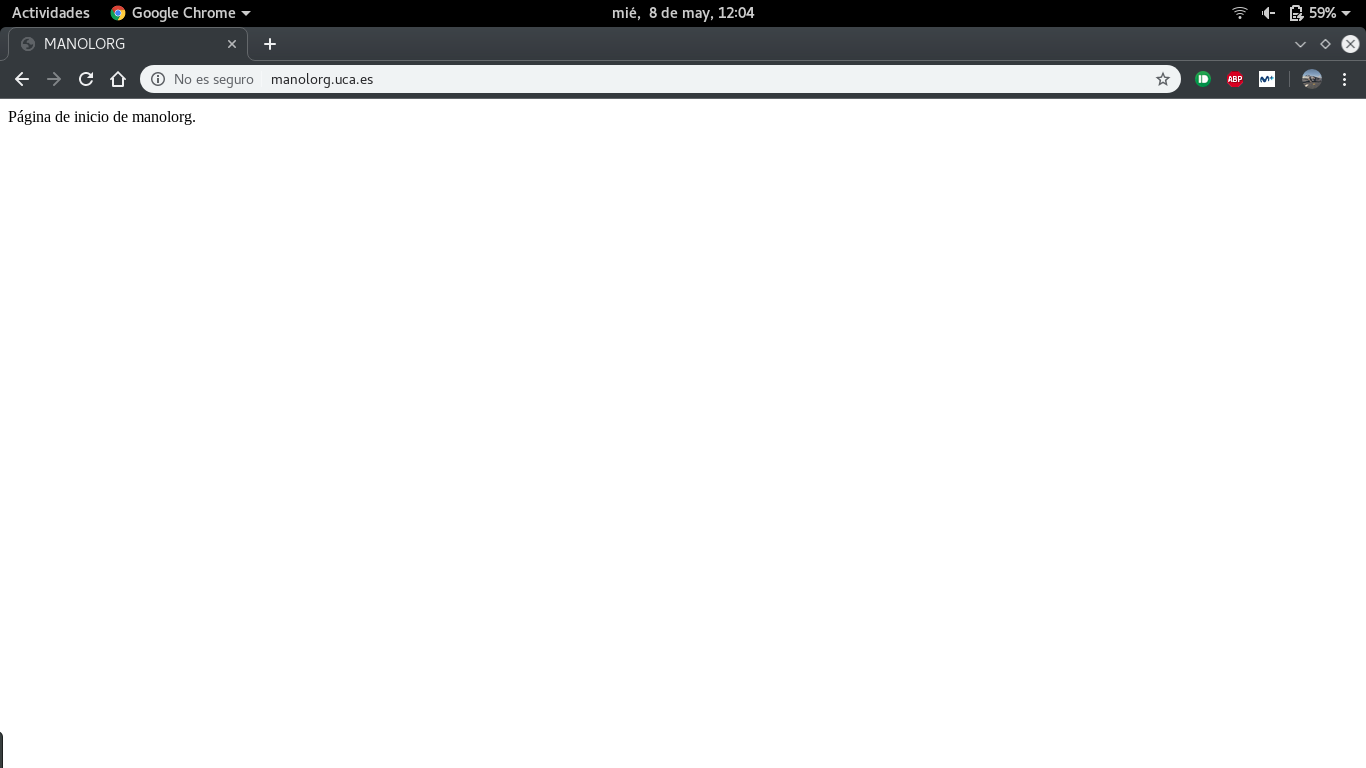
\includegraphics[scale=0.34]{ConUTF8.png}
	\caption{Con UTF8}
	\label{Con UTF8}
\end{figure}

\section{Caché}
Las imágenes (png, jpg) se cachearán para agilizar la web (hay muchas fotos). Esto se hará por medio del plugin expires.

Para ello, iremos a ``Configure Apache Modules'' y seleccionamos la opción ``Expires''.

Para descargar la imagen usar el siguiente comando:
\begin{center}
	\texttt{wget dirección}
\end{center}

Y la ubicaremos en el ``Document root'' del servidor\footnote{La hemos renombrado como \texttt{UCA.jpg} para que sea más corto.}.

Siendo \texttt{dirección}, la dirección de la imagen.

Para configurar la expiración de la caché, nos dirigimos al ``Edit directives'' del virtual host (\texttt{manolorg.uca.es}) y añadimos en el apartado de dicho directorio el siguiente código:
\begin{center}
	\texttt{ExpiresActive On\\
		ExpiresByType image/jpeg ``access plus 3 minutes''}
\end{center}

Para comprobar si funciona abrimos una consola en nuestro ordenador y ejecutamos el comando:
\begin{center}
	\texttt{curl ---head manolorg.uca.es/UCA.jpg}
\end{center}

\newpage
Una vez hecho eso, obtenemos lo siguiente:
\begin{figure}[h]
	\centering
	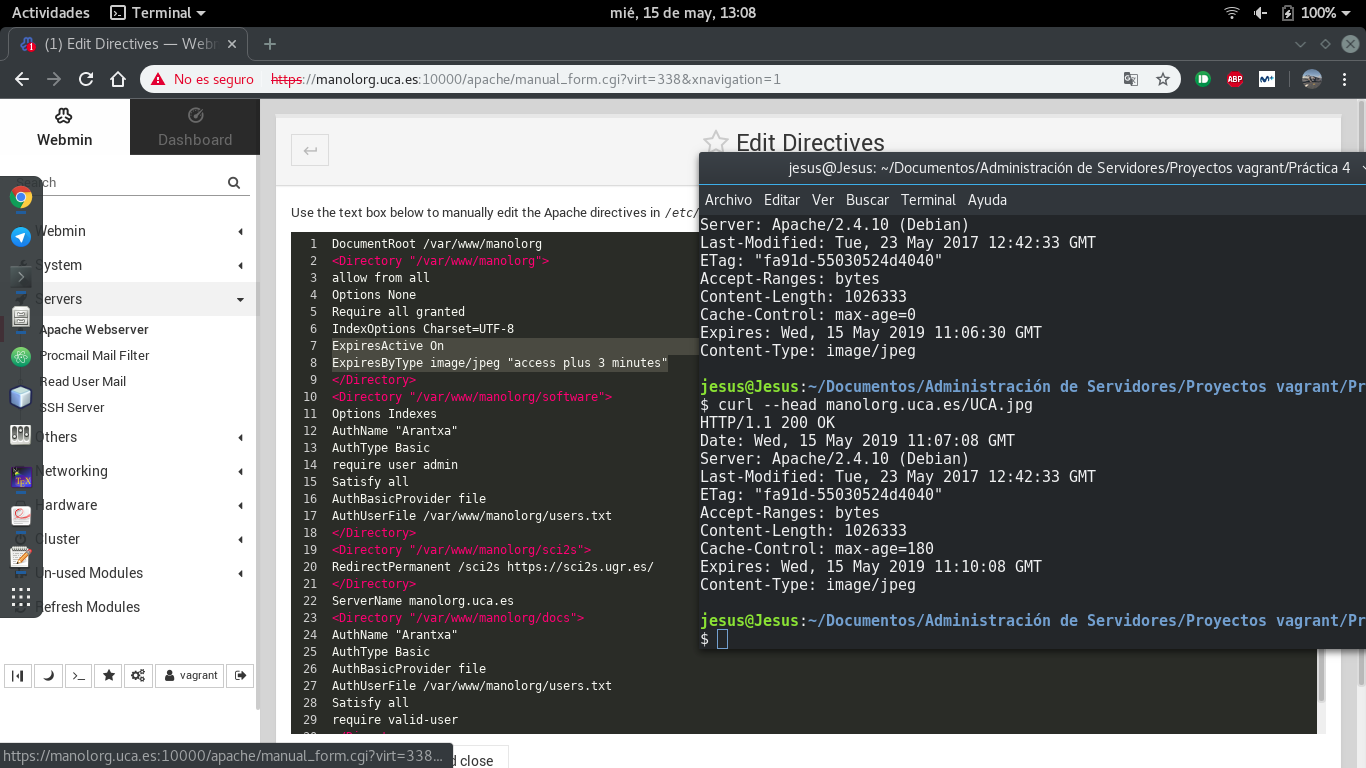
\includegraphics[scale=0.34]{Expires.png}
	\caption{Configuración y resultado del expires.}
	\label{Configuración y resultado del expires}
\end{figure}

\section{Redirección}
\begin{itemize}
	\item Hay un problema en la base de datos con los nombres, y algunos ficheros aparecen erróneamente como .jpeg de forma errónea. Se desea que en el subdirectorio /imagenes todos los
	ficheros con extensión .jpeg se busquen con extensión .jpg.
	
	Para ello, creamos el subdirectorio \texttt{/imagenes} en el directorio \texttt{/var/www/manolorg}.
	
	A continuación, creamos el directory \texttt{/imagenes} en webmin.
	
	En ``Global configuration'' nos vamos a ``Configure Apache Modules'' y activamos el módulo \texttt{rewrite}.
	
	Luego, nos dirigimos al ``Edit directives'' de \texttt{manolorg} y añadimos al final lo siguiente:
	\begin{center}
		\texttt{RewriteEngine On\\
			RewriteRule ``\^/imagenes/(.*)\.jpeg'' ``/imagenes/\$1.jpg'' [R]}
		\\Es un acento circunflejo.
	\end{center}

	Entonces, al buscar \texttt{http://manolorg.uca.es/imagenes/UCA.jpeg}, nos mostrará \texttt{http://manolorg.uca.es/imagenes/UCA.jpg} y nos cambiará la dirección como podemos ver en la siguiente imagen.
	\newpage
	\begin{figure}[h]
		\centering
		
\includegraphics[scale=0.34]{Imagen.png}
		\caption{Imagen del subdirectorio imágenes.}
		\label{Imagen}
	\end{figure}
	
	\item Modificar la condición anterior para que sólo cambie las extensiones a .jpg cuando no exista el fichero con la extensión .jpeg.

	Para ello tendremos que añadir una condición al ``Edit directives'' del ``Global configuration'' poniéndole lo siguiente:
	\begin{center}
		\texttt{RewriteCond \%{Document\_root}\%{Request\_Filename} !-f}
	\end{center}
	
	Luego, probamos a entrar en: \texttt{http://manolorg.uca.es/imagenes/UCA2.jpeg} y nos mostrará la ``jpeg'' aunque exista la ``jpg''.
	\newpage
	\begin{figure}[h]
		\centering
		
\includegraphics[scale=0.34]{Imagen2.png}
		\caption{Imagen jpeg.}
		\label{Imagen jpeg}
	\end{figure}
	
	\item El dominio manologr.uca.es tiene diferentes páginas para cada usuario. Estás páginas se sirven de forma dinámica mediante php. Así, la URL manologr.uca.es/personalWeb.php?user=\\CoboMJ mostrará la página personal del usuario CoboMJ donde se podría ver el listado de sus	publicaciones. Necesitamos convertir esta URL en una URL más ambigable del tipo manolo.uca.es/team/CoboMJ. Para poder probar el funcionamiento, se deberá crear la página php personalWeb.php que lo único que hará es mostrar un mensaje con el parámetro pasado por get.
	
	Para ello, crearemos el fichero \texttt{personalWeb.php} en \texttt{/var/www/manolorg/} con un get:
	\begin{lstlisting}{language=php}
		<?php
		echo '¡Hola ' . htmlspecialchars($_GET["user"]) . '!';
		?>
	\end{lstlisting}
	
	Ahora probamos a entrar en \texttt{http://manolorg.uca.es/personalWeb.php?user=JAR} y veremos lo siguiente:
	\newpage
	\begin{figure}[h]
		\centering
		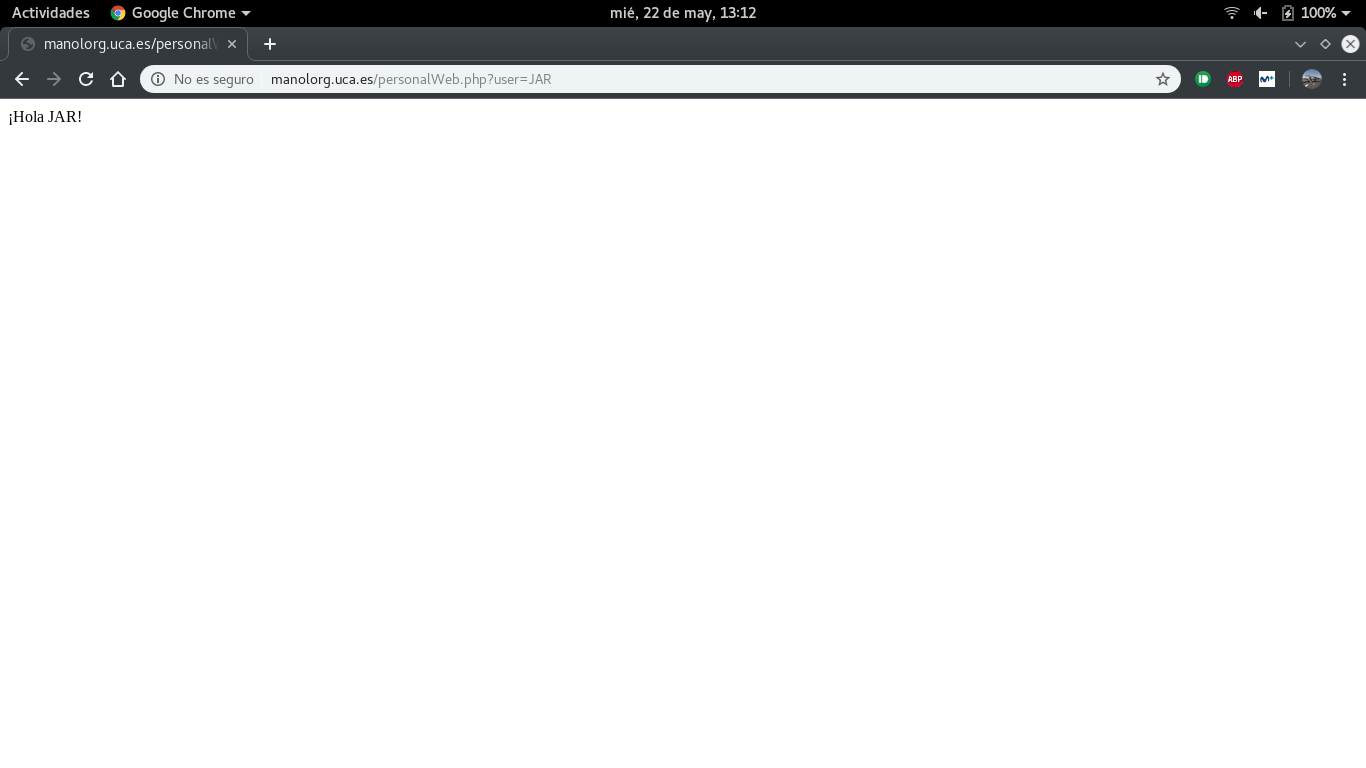
\includegraphics[scale=0.34]{JAR.png}
		\caption{Comprobación php.}
		\label{Comprobación php}
	\end{figure}

	Ahora, añadimos la siguiente línea en el ``Edit directives'' de ``Global configuration'':
	\begin{center}
		\texttt{RewriteRule ``\^/team/(.*)'' ``/personalWeb.php?user=\$1''}
	\end{center}
	
	Para comprobar que funciona nos dirigimos a la siguiente dirección:\\ \texttt{manolorg.uca.es/team/JAR2}, y nos sale lo siguiente:
	\newpage
	\begin{figure}[h]
		\centering
		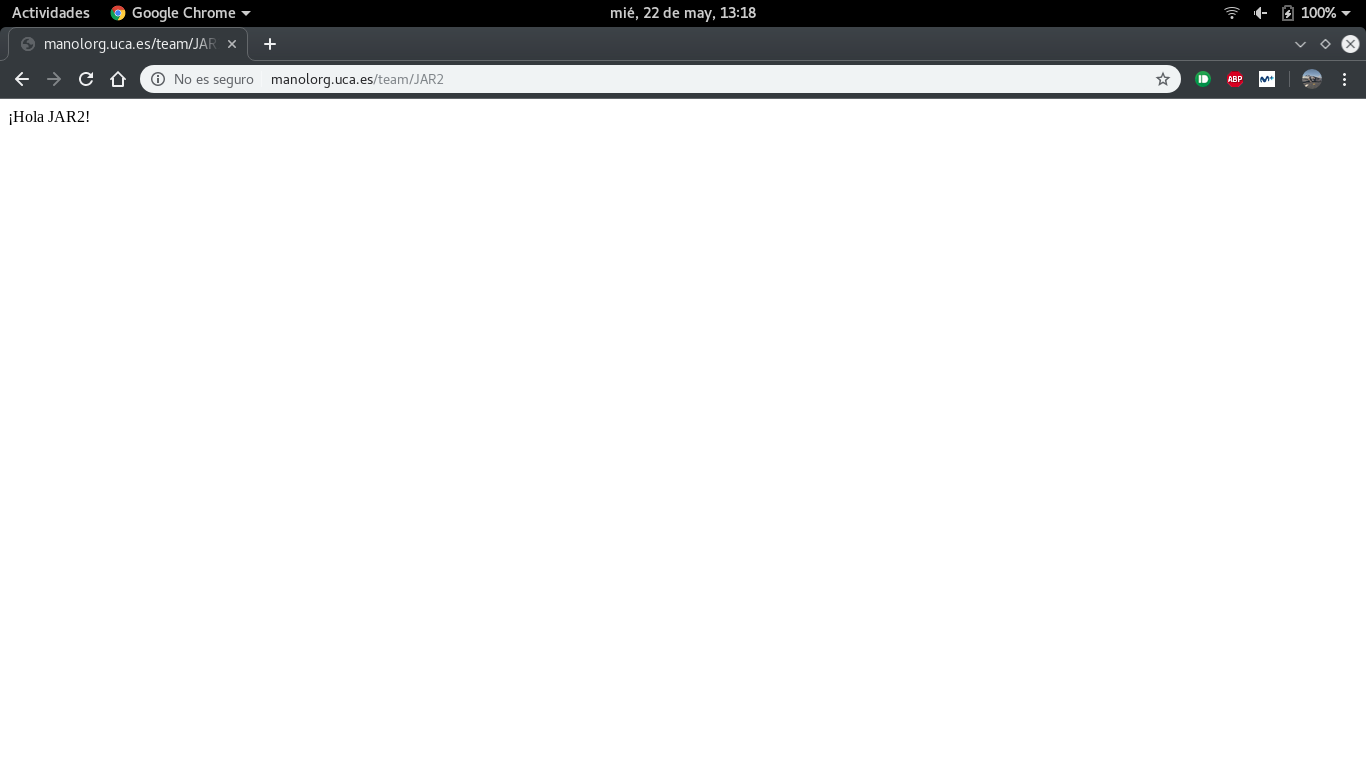
\includegraphics[scale=0.34]{JAR2.png}
		\caption{Comprobación de php con redirección.}
		\label{PHP2}
	\end{figure}
\end{itemize}

\section{Balanceo de carga}


\end{document}